\documentclass[a4paper]{article}
\usepackage[]{graphicx}\usepackage[]{color}
% maxwidth is the original width if it is less than linewidth
% otherwise use linewidth (to make sure the graphics do not exceed the margin)
\makeatletter
\def\maxwidth{ %
  \ifdim\Gin@nat@width>\linewidth
    \linewidth
  \else
    \Gin@nat@width
  \fi
}
\makeatother

\definecolor{fgcolor}{rgb}{0.345, 0.345, 0.345}
\newcommand{\hlnum}[1]{\textcolor[rgb]{0.686,0.059,0.569}{#1}}%
\newcommand{\hlstr}[1]{\textcolor[rgb]{0.192,0.494,0.8}{#1}}%
\newcommand{\hlcom}[1]{\textcolor[rgb]{0.678,0.584,0.686}{\textit{#1}}}%
\newcommand{\hlopt}[1]{\textcolor[rgb]{0,0,0}{#1}}%
\newcommand{\hlstd}[1]{\textcolor[rgb]{0.345,0.345,0.345}{#1}}%
\newcommand{\hlkwa}[1]{\textcolor[rgb]{0.161,0.373,0.58}{\textbf{#1}}}%
\newcommand{\hlkwb}[1]{\textcolor[rgb]{0.69,0.353,0.396}{#1}}%
\newcommand{\hlkwc}[1]{\textcolor[rgb]{0.333,0.667,0.333}{#1}}%
\newcommand{\hlkwd}[1]{\textcolor[rgb]{0.737,0.353,0.396}{\textbf{#1}}}%
\let\hlipl\hlkwb

\usepackage{framed}
\makeatletter
\newenvironment{kframe}{%
 \def\at@end@of@kframe{}%
 \ifinner\ifhmode%
  \def\at@end@of@kframe{\end{minipage}}%
  \begin{minipage}{\columnwidth}%
 \fi\fi%
 \def\FrameCommand##1{\hskip\@totalleftmargin \hskip-\fboxsep
 \colorbox{shadecolor}{##1}\hskip-\fboxsep
     % There is no \\@totalrightmargin, so:
     \hskip-\linewidth \hskip-\@totalleftmargin \hskip\columnwidth}%
 \MakeFramed {\advance\hsize-\width
   \@totalleftmargin\z@ \linewidth\hsize
   \@setminipage}}%
 {\par\unskip\endMakeFramed%
 \at@end@of@kframe}
\makeatother

\definecolor{shadecolor}{rgb}{.97, .97, .97}
\definecolor{messagecolor}{rgb}{0, 0, 0}
\definecolor{warningcolor}{rgb}{1, 0, 1}
\definecolor{errorcolor}{rgb}{1, 0, 0}
\newenvironment{knitrout}{}{} % an empty environment to be redefined in TeX

\usepackage{alltt}
\newcommand{\SweaveOpts}[1]{}  % do not interfere with LaTeX
\newcommand{\SweaveInput}[1]{} % because they are not real TeX commands
\newcommand{\Sexpr}[1]{}       % will only be parsed by R




\usepackage[utf8]{inputenc}
%\usepackage[ngerman]{babel}
\usepackage{a4wide,paralist}
\usepackage{amsmath, amssymb, xfrac, amsthm}
\usepackage{dsfont}
\usepackage[usenames,dvipsnames]{xcolor}
\usepackage{amsfonts}
\usepackage{graphicx}
\usepackage{caption}
\usepackage{subcaption}
\usepackage{framed}
\usepackage{multirow}
\usepackage{bytefield}
\usepackage{csquotes}
\usepackage[breakable, theorems, skins]{tcolorbox}
\usepackage{hyperref}
\usepackage{cancel}
\usepackage{bm}


\usepackage{bbm}
% basic latex stuff
\newcommand{\pkg}[1]{{\fontseries{b}\selectfont #1}} %fontstyle for R packages
\newcommand{\lz}{\vspace{0.5cm}} %vertical space
\newcommand{\dlz}{\vspace{1cm}} %double vertical space
\newcommand{\oneliner}[1] % Oneliner for important statements
{\begin{block}{}\begin{center}\begin{Large}#1\end{Large}\end{center}\end{block}}


%new environments
\newenvironment{vbframe}  %frame with breaks and verbatim
{
 \begin{frame}[containsverbatim,allowframebreaks]
}
{
\end{frame}
}

\newenvironment{vframe}  %frame with verbatim without breaks (to avoid numbering one slided frames)
{
 \begin{frame}[containsverbatim]
}
{
\end{frame}
}

\newenvironment{blocki}[1]   % itemize block
{
 \begin{block}{#1}\begin{itemize}
}
{
\end{itemize}\end{block}
}

\newenvironment{fragileframe}[2]{  %fragile frame with framebreaks
\begin{frame}[allowframebreaks, fragile, environment = fragileframe]
\frametitle{#1}
#2}
{\end{frame}}


\newcommand{\myframe}[2]{  %short for frame with framebreaks
\begin{frame}[allowframebreaks]
\frametitle{#1}
#2
\end{frame}}

\newcommand{\remark}[1]{
  \textbf{Remark:} #1
}

\newcommand{\citebutton}[2]{%
\NoCaseChange{\resizebox{!}{9pt}{\protect\beamergotobutton{\href{#2}{#1}}}}%
}



\newenvironment{deleteframe}
{
\begingroup
\usebackgroundtemplate{\includegraphics[width=\paperwidth,height=\paperheight]{../style/color/red.png}}
 \begin{frame}
}
{
\end{frame}
\endgroup
}
\newenvironment{simplifyframe}
{
\begingroup
\usebackgroundtemplate{\includegraphics[width=\paperwidth,height=\paperheight]{../style/color/yellow.png}}
 \begin{frame}
}
{
\end{frame}
\endgroup
}\newenvironment{draftframe}
{
\begingroup
\usebackgroundtemplate{\includegraphics[width=\paperwidth,height=\paperheight]{../style/color/green.jpg}}
 \begin{frame}
}
{
\end{frame}
\endgroup
}
% https://tex.stackexchange.com/a/261480: textcolor that works in mathmode
\makeatletter
\renewcommand*{\@textcolor}[3]{%
  \protect\leavevmode
  \begingroup
    \color#1{#2}#3%
  \endgroup
}
\makeatother


\tcbset{enhanced}

\DeclareRobustCommand{\mybox}[2][gray!20]{%
	\iffalse
	\begin{tcolorbox}[   %% Adjust the following parameters at will.
		breakable,
		left=0pt,
		right=0pt,
		top=0pt,
		bottom=0pt,
		colback=#1,
		colframe=#1,
		width=\dimexpr\linewidth\relax,
		enlarge left by=0mm,
		boxsep=5pt,
		arc=0pt,outer arc=0pt,
		]
		#2
	\end{tcolorbox}
	\fi
}

\DeclareRobustCommand{\myboxshow}[2][gray!20]{%
%	\iffalse
	\begin{tcolorbox}[   %% Adjust the following parameters at will.
		breakable,
		left=0pt,
		right=0pt,
		top=0pt,
		bottom=0pt,
		colback=#1,
		colframe=#1,
		width=\dimexpr\linewidth\relax,
		enlarge left by=0mm,
		boxsep=5pt,
		arc=0pt,outer arc=0pt,
		]
		#2
	\end{tcolorbox}
%	\fi
}


%exercise numbering
\renewcommand{\theenumi}{(\alph{enumi})}
\renewcommand{\theenumii}{\roman{enumii}}
\renewcommand\labelenumi{\theenumi}


\font \sfbold=cmssbx10

\setlength{\oddsidemargin}{0cm} \setlength{\textwidth}{16cm}


\sloppy
\parindent0em
\parskip0.5em
\topmargin-2.3 cm
\textheight25cm
\textwidth17.5cm
\oddsidemargin-0.8cm
\pagestyle{empty}

\newcommand{\kopf}[1] {
\hrule
\vspace{.15cm}
\begin{minipage}{\textwidth}
%akwardly i had to put \" here to make it compile correctly
	{\sf\bf Introduction to Machine Learning \hfill #1. Exercise\\
	 \url{https://introduction-to-machine-learning.netlify.app/} \hfill WiSe 2020/2021}
\end{minipage}
\vspace{.05cm}
\hrule
\vspace{1cm}}

\newenvironment{allgemein}
	{\noindent}{\vspace{1cm}}

\newcounter{aufg}
\newenvironment{aufgabe}
	{\refstepcounter{aufg}\textbf{Exercise \arabic{aufg}:}\\ \noindent}
	{\vspace{0.5cm}}

\newenvironment{loesung}
	{\refstepcounter{aufg}\textbf{Solution \arabic{aufg}:}\\\noindent}
	{\bigskip}
	
\newenvironment{bonusaufgabe}
	{\refstepcounter{aufg}\textbf{Exercise \arabic{aufg}*\footnote{This
	is a bonus exercise.}:}\\ \noindent}
	{\vspace{0.5cm}}

\newenvironment{bonusloesung}
	{\refstepcounter{aufg}\textbf{Solution \arabic{aufg}*:}\\\noindent}
	{\bigskip}



\begin{document}
% !Rnw weave = knitr




\kopf{3}

\loesung{

\begin{itemize}
\item The inner loss is the loss that is optimized directly by the machine learning model. 
The outer loss is the loss (or performance measurement) used to evaluate the model.
\item Which model is more likely to overfit the training data: 
\begin{itemize}
\item k-NN with 1 or with 10 neighbors? \textbf{1 neighbor}, because it's an exact memorization of training data. 
\item Logistic regression with 10 or 20 features? \textbf{20 features}, because the more features, the more coefficients the learner estimates. More coefficients mean more degrees of freedom, which make overfitting more likely.
\item LDA or QDA? \textbf{QDA}, because it has more parameters to possibly overfit the data. LDA is more likely to underfit more complex relationships.
\end{itemize}
\item Which of the following methods yield an unbiased generalization error estimate? Performance estimation ...
\begin{itemize}
  \item  on training data: \textbf{Biased, too optimistic}
  \item  on test data:  \textbf{Unbiased / Biased, too pessimistic} (Test data is \textit{not included} / \textit{included} in the final model)
  \item  on training and test data combined: \textbf{Biased, too optimistic} (But a little bit less than only using training data).
  \item  using cross validation: \textbf{Biased, too pessimistic} (The higher the ratio of folds / number of observation, the smaller the pessimistic bias)
  \item  using subsampling: \textbf{Biased, too pessimistic} (The smaller the subsampling rate, the larger the pessimistic bias)
\end{itemize}
\item Resampling strategies solve the problem that comes from the randomness of the training and test data split: Error estimation using a single split has a high variance. Resampling estimates are more robust because they average over different splits.
\item Nested resampling solves the problem of simultaneously conducting tuning/model selection and performance estimation. When we use the performance estimates from the same data that were used for model selection (as done in simple, not-nested resampling), the final error estimate is too optimistic.
\end{itemize}
}

\dlz

\loesung{

\begin{itemize}
\item The training performance is too optimistic  (mmce of 0), because the mmce is higher on new data.
\item The test performance is unbiased (if the final model is only trained on the training data), but it depends on the split, as can be seen in the CV folds: 
  Each CV fold represents a training test split and the mmce measure varies between folds.
\item The CV estimate averages over the different splits and gives an slightly pessimistic, more robust estimate.
\item The CV estimate is preferable over the other two, but more computationally expensive.
\end{itemize}
}

\pagebreak[4]

\dlz

\loesung{



\begin{enumerate}
  \item[a)]

  Each loss function we have learned so far to fit the model (inner loss) can also be used as performance measure (outer loss).

  For classification:

  \begin{itemize}
    \item 0-1 loss (= mean misclassification error),
    \item Logistic loss (bernoulli loss), ...
  \end{itemize}

  For regression:

  \begin{itemize}
    \item $L_2$-loss (= mean squared error),
    \item $L_1$-loss (= mean absolute error), ...
  \end{itemize}

  To get a list of all measures you can use \texttt{mlr\_measures}.

  \item[b)]

\begin{knitrout}
\definecolor{shadecolor}{rgb}{0.969, 0.969, 0.969}\color{fgcolor}\begin{kframe}
\begin{alltt}
\hlcom{# look at the task}
\hlstd{task} \hlkwb{<-} \hlkwd{tsk}\hlstd{(}\hlstr{"boston_housing"}\hlstd{)}
\hlstd{task}
\end{alltt}
\begin{verbatim}
## <TaskRegr:boston_housing> (506 x 19)
## * Target: medv
## * Properties: -
## * Features (18):
##   - dbl (13): age, b, cmedv, crim, dis, indus, lat, lon, lstat, nox,
##     ptratio, rm, zn
##   - int (3): rad, tax, tract
##   - fct (2): chas, town
\end{verbatim}
\begin{alltt}
\hlstd{n} \hlkwb{<-} \hlstd{task}\hlopt{$}\hlstd{nrow}

\hlcom{# select index vectors to subset the data randomly}
\hlkwd{set.seed}\hlstd{(}\hlnum{123}\hlstd{)}
\hlstd{train_ind} \hlkwb{<-} \hlkwd{sample}\hlstd{(}\hlkwd{seq_len}\hlstd{(n),} \hlnum{0.5}\hlopt{*}\hlstd{n)}
\hlstd{test_ind} \hlkwb{<-} \hlkwd{setdiff}\hlstd{(}\hlkwd{seq_len}\hlstd{(n), train_ind)}

\hlcom{# specify learner}
\hlstd{learner} \hlkwb{<-} \hlkwd{lrn}\hlstd{(}\hlstr{"regr.kknn"}\hlstd{,} \hlkwc{k} \hlstd{=} \hlnum{3}\hlstd{)}

\hlcom{# train model to the training set}
\hlstd{learner}\hlopt{$}\hlkwd{train}\hlstd{(task,} \hlkwc{row_ids} \hlstd{= train_ind)}

\hlcom{# predict on the test set}
\hlstd{pred} \hlkwb{<-} \hlstd{learner}\hlopt{$}\hlkwd{predict}\hlstd{(task,} \hlkwc{row_ids} \hlstd{= test_ind)}
\hlstd{pred}
\end{alltt}
\begin{verbatim}
## <PredictionRegr> for 253 observations:
##     row_ids truth response
##           1  24.0 23.22445
##           2  21.6 19.98830
##           3  34.7 34.97419
## ---                       
##         504  23.9 22.22775
##         505  22.0 21.76531
##         506  11.9 20.88958
\end{verbatim}
\end{kframe}
\end{knitrout}
  \item[c)]
\begin{knitrout}
\definecolor{shadecolor}{rgb}{0.969, 0.969, 0.969}\color{fgcolor}\begin{kframe}
\begin{alltt}
\hlcom{# predict on the train set}
\hlstd{pred_train} \hlkwb{<-} \hlstd{learner}\hlopt{$}\hlkwd{predict}\hlstd{(task,} \hlkwc{row_ids} \hlstd{= train_ind)}
\hlstd{pred_train}\hlopt{$}\hlkwd{score}\hlstd{(}\hlkwd{list}\hlstd{(}\hlkwd{msr}\hlstd{(}\hlstr{"regr.mse"}\hlstd{),} \hlkwd{msr}\hlstd{(}\hlstr{"regr.mae"}\hlstd{)))}
\end{alltt}
\begin{verbatim}
##  regr.mse  regr.mae 
## 1.2322560 0.7564092
\end{verbatim}
\begin{alltt}
\hlcom{# predict on the test set}
\hlstd{pred_test} \hlkwb{<-} \hlstd{learner}\hlopt{$}\hlkwd{predict}\hlstd{(task,} \hlkwc{row_ids} \hlstd{= test_ind)}
\hlstd{pred_test}\hlopt{$}\hlkwd{score}\hlstd{(}\hlkwd{list}\hlstd{(}\hlkwd{msr}\hlstd{(}\hlstr{"regr.mse"}\hlstd{),} \hlkwd{msr}\hlstd{(}\hlstr{"regr.mae"}\hlstd{)))}
\end{alltt}
\begin{verbatim}
##  regr.mse  regr.mae 
## 12.424958  2.596332
\end{verbatim}
\end{kframe}
\end{knitrout}
  Unsurprisingly the model performs better on the training data (smaller loss) then on the
  test data.

  \item[d)]

\begin{knitrout}
\definecolor{shadecolor}{rgb}{0.969, 0.969, 0.969}\color{fgcolor}\begin{kframe}
\begin{alltt}
\hlcom{# select different index vectors to subset the data randomly}
\hlkwd{set.seed}\hlstd{(}\hlnum{321}\hlstd{)}
\hlstd{train_ind} \hlkwb{<-} \hlkwd{sample}\hlstd{(}\hlkwd{seq_len}\hlstd{(n),} \hlnum{0.5}\hlopt{*}\hlstd{n)}
\hlstd{test_ind} \hlkwb{<-} \hlkwd{setdiff}\hlstd{(}\hlkwd{seq_len}\hlstd{(n), train_ind)}

\hlcom{# specify learner}
\hlstd{learner} \hlkwb{<-} \hlkwd{lrn}\hlstd{(}\hlstr{"regr.kknn"}\hlstd{,} \hlkwc{k} \hlstd{=} \hlnum{3}\hlstd{)}

\hlcom{# train model to the training set}
\hlstd{learner}\hlopt{$}\hlkwd{train}\hlstd{(task,} \hlkwc{row_ids} \hlstd{= train_ind)}

\hlcom{# predict on the test set}
\hlstd{pred_test} \hlkwb{<-} \hlstd{learner}\hlopt{$}\hlkwd{predict}\hlstd{(task,} \hlkwc{row_ids} \hlstd{= test_ind)}
\hlstd{pred_test}
\end{alltt}
\begin{verbatim}
## <PredictionRegr> for 253 observations:
##     row_ids truth response
##           2  21.6 29.45474
##           5  36.2 33.14900
##           6  28.7 32.95574
## ---                       
##         501  16.8 19.61312
##         505  22.0 23.29286
##         506  11.9 21.28301
\end{verbatim}
\begin{alltt}
\hlstd{pred_test}\hlopt{$}\hlkwd{score}\hlstd{(}\hlkwd{list}\hlstd{(}\hlkwd{msr}\hlstd{(}\hlstr{"regr.mse"}\hlstd{),} \hlkwd{msr}\hlstd{(}\hlstr{"regr.mae"}\hlstd{)))}
\end{alltt}
\begin{verbatim}
##  regr.mse  regr.mae 
## 12.507468  2.458798
\end{verbatim}
\end{kframe}
\end{knitrout}

  Effect: We will predict different observations since the test set is different. The same observations get a slightly different prediction (e.g. observation with id 2). This affects the final error estimation.

  \item[e)]
\begin{knitrout}
\definecolor{shadecolor}{rgb}{0.969, 0.969, 0.969}\color{fgcolor}\begin{kframe}
\begin{alltt}
\hlstd{rdesc} \hlkwb{<-} \hlkwd{rsmp}\hlstd{(}\hlstr{"cv"}\hlstd{,} \hlkwc{folds} \hlstd{=} \hlnum{10}\hlstd{)}
\hlstd{r} \hlkwb{<-} \hlkwd{resample}\hlstd{(task, learner, rdesc)}
\end{alltt}
\begin{verbatim}
## INFO  [09:28:20.256] [mlr3]  Applying learner 'regr.kknn' on task 'boston_housing' (iter 9/10) 
## INFO  [09:28:20.305] [mlr3]  Applying learner 'regr.kknn' on task 'boston_housing' (iter 10/10) 
## INFO  [09:28:20.330] [mlr3]  Applying learner 'regr.kknn' on task 'boston_housing' (iter 7/10) 
## INFO  [09:28:20.349] [mlr3]  Applying learner 'regr.kknn' on task 'boston_housing' (iter 6/10) 
## INFO  [09:28:20.368] [mlr3]  Applying learner 'regr.kknn' on task 'boston_housing' (iter 4/10) 
## INFO  [09:28:20.390] [mlr3]  Applying learner 'regr.kknn' on task 'boston_housing' (iter 8/10) 
## INFO  [09:28:20.413] [mlr3]  Applying learner 'regr.kknn' on task 'boston_housing' (iter 1/10) 
## INFO  [09:28:20.436] [mlr3]  Applying learner 'regr.kknn' on task 'boston_housing' (iter 5/10) 
## INFO  [09:28:20.456] [mlr3]  Applying learner 'regr.kknn' on task 'boston_housing' (iter 3/10) 
## INFO  [09:28:20.476] [mlr3]  Applying learner 'regr.kknn' on task 'boston_housing' (iter 2/10)
\end{verbatim}
\begin{alltt}
\hlstd{r}\hlopt{$}\hlkwd{aggregate}\hlstd{(}\hlkwd{list}\hlstd{(}\hlkwd{msr}\hlstd{(}\hlstr{"regr.mse"}\hlstd{),} \hlkwd{msr}\hlstd{(}\hlstr{"regr.mae"}\hlstd{)))}
\end{alltt}
\begin{verbatim}
##  regr.mse  regr.mae 
## 10.045363  2.229458
\end{verbatim}
\end{kframe}
\end{knitrout}

  % \item[f)]
  % <<message=FALSE>>=
  % ## Tuning in inner resampling loop
  % ps = makeParamSet(makeDiscreteParam("k", values = 1:10))
  % ctrl = makeTuneControlGrid()
  % inner = makeResampleDesc("CV", iters = 10)
  % lrn = makeTuneWrapper("regr.kknn", resampling = inner, par.set = ps, control = ctrl, show.info = FALSE)

  % ## Outer resampling loop
  % outer = makeResampleDesc("CV", iters = 5)
  % r = resample(lrn, bh.task, resampling = outer, extract = getTuneResult, show.info = FALSE)
  % r$measures.test
  % r$aggr
  % r$extract
  % @
\end{enumerate}
}

\dlz

\loesung{

\begin{enumerate}
  \item[a)] First, sort the table:
  \begin{center}
  \begin{tabular}{ | c | c | c | c |}
  \hline
  ID & Actual Class & Score & Predicted Class \\ \hline
  6 & 0 & 0.63 & 1  \\
  7 & 1 & 0.62 & 1  \\
  10 & 0 & 0.57 & 1 \\
  \hline
  4 & 1 & 0.38 & 0  \\
  1 & 0 & 0.33 & 0  \\
  8 & 1 & 0.33 & 0  \\
  2 & 0 & 0.27 & 0  \\
  5 & 1 & 0.17 & 0  \\
  9 & 0 & 0.15 & 0 \\
  3 & 1 & 0.11 & 0  \\
  \hline\text{
  }  \end{tabular}
  \end{center}


  \begin{center}
  \begin{tabular}{ | c | c | c | }
  \hline
   & Actual Class - 0 & Actual Class - 1  \\
  Prediction - 0 & 3 & 4  \\
  Prediction - 1 & 2 & 1  \\
      \hline
    \end{tabular}
  \end{center}

  so we get

  \begin{center}
  \begin{tabular}{ | c | c | c | c | }
  \hline
  FN & FP & TN & TP   \\ \hline
  4 & 2 & 3 & 1 \\
      \hline
    \end{tabular}
  \end{center}

  \item[b)]

  $$\text{Precision} = \frac{\text{TP}}{\text{TP} + \text{FP}} =\frac{1}{3} $$

  $$\text{Sensitivity} = \frac{\text{TP}}{\text{TP} + \text{FN}} =\frac{1}{5} $$

  $$\text{Accuracy} = \frac{\text{TP} + \text{TN}}{\text{TP} + \text{TN} + \text{FP} + \text{FN}} =\frac{4}{10} $$

  $$\text{Specificity}  = \frac{\text{TN}}{\text{TN} + \text{FP}} =\frac{3}{5} $$

  $$\text{Error Rate}  = \frac{\text{FP} + \text{FN}}{\text{TP} + \text{TN} + \text{FP} + \text{FN}} =\frac{6}{10} $$

  $$\text{F-measure} = \frac{2\cdot\text{Precision}\cdot\text{Sensitivity}}{\text{Precision}+\text{Sensitivity}} = 0.25 $$

  $$\text{Negative Predictive Value} = \frac{\text{TN}}{\text{TN} + \text{FN}} =\frac{3}{7} $$

  \item[c)] 
First we sort the results by the score: \\
\begin{knitrout}
\definecolor{shadecolor}{rgb}{0.969, 0.969, 0.969}\color{fgcolor}
\begin{tabular}{l|r|r}
\hline
  & true\_labels & scores\\
\hline
6 & 0 & 0.63\\
\hline
7 & 1 & 0.62\\
\hline
10 & 0 & 0.57\\
\hline
4 & 1 & 0.38\\
\hline
1 & 0 & 0.33\\
\hline
8 & 1 & 0.33\\
\hline
2 & 0 & 0.27\\
\hline
5 & 1 & 0.17\\
\hline
9 & 0 & 0.15\\
\hline
3 & 1 & 0.10\\
\hline
\end{tabular}

\end{knitrout}
Here we see that $\frac{1}{n_+} = \frac{1}{5} = 0.2$ and $\frac{1}{n_-} = \frac{1}{5} = 0.2$. Now we follow the algorithm as described in the lecture slides:
\begin{enumerate}
\item Set $\alpha = 1$, so we start in $(0,0)$; we predict everything as 1.
\item Set threshold $\tau = 0.625$ yields TPR 0 and FPR  $0 + \frac{1}{n_-} = 0.2$. (Obs. 6 is "0")
\item Set threshold $\tau = 0.6$ yields TPR $0 + \frac{1}{n_+} = 0.2$ and FPR  $0.2$. (Obs. 7 is "1")
\item Set threshold $\tau = 0.5$ yields TPR 0.2 and FPR  $0.2 + \frac{1}{n_-} = 0.4$. (Obs. 10 is "0")
\item Set threshold $\tau = 0.35$ yields TPR $0.2 + \frac{1}{n_+} = 0.4$ and FPR  $0.4$. (Obs. 4 is "1")
\item Set threshold $\tau = 0.3$ yields TPR $0.4 + \frac{1}{n_+} = 0.6$ and FPR  $0.4 + \frac{1}{n_-} = 0.6$. (Obs. 1/8 is "0"/"1")
\item Set threshold $\tau = 0.2$ yields TPR $0.6$ and FPR  $0.6 + \frac{1}{n_-} = 0.8$. (Obs. 2 is "0")
\item Set threshold $\tau = 0.16$ yields TPR $0.6 + \frac{1}{n_+} = 0.8$ and FPR  $0.8$. (Obs. 5 is "1")
\item Set threshold $\tau = 0.14$ yields TPR $0.8$ and FPR  $0.8 + \frac{1}{n_-} = 1$. (Obs. 9 is "0")
\item Set threshold $\tau = 0.09$ yields TPR $0.8 + \frac{1}{n_+} = 1$ and FPR  $1$. (Obs. 3 is "1")
\end{enumerate}

Therefore we get the polygonal path consisting of the ordered list of vertices \[(0,0), (0.2,0), (0.2,0.2),
(0.4,0.2), (0.4,0.4), (0.6,0.6), (0.8,0.6), (0.8, 0.8), (1, 0.8), (1,1).\]

\begin{knitrout}
\definecolor{shadecolor}{rgb}{0.969, 0.969, 0.969}\color{fgcolor}\begin{kframe}
\begin{alltt}
\hlkwd{library}\hlstd{(ggplot2)}
\hlstd{roc_data} \hlkwb{<-} \hlkwd{data.frame}\hlstd{(}\hlkwc{TPR} \hlstd{=} \hlkwd{c}\hlstd{(}\hlnum{0}\hlstd{,} \hlnum{0}\hlstd{,}   \hlnum{0.2}\hlstd{,} \hlnum{0.2}\hlstd{,} \hlnum{0.4}\hlstd{,} \hlnum{0.6}\hlstd{,} \hlnum{0.6}\hlstd{,} \hlnum{0.8}\hlstd{,} \hlnum{0.8}\hlstd{,} \hlnum{1}\hlstd{),}
                       \hlkwc{FPR} \hlstd{=} \hlkwd{c}\hlstd{(}\hlnum{0}\hlstd{,} \hlnum{0.2}\hlstd{,} \hlnum{0.2}\hlstd{,} \hlnum{0.4}\hlstd{,} \hlnum{0.4}\hlstd{,} \hlnum{0.6}\hlstd{,} \hlnum{0.8}\hlstd{,} \hlnum{0.8}\hlstd{,}  \hlnum{1}\hlstd{,}  \hlnum{1}\hlstd{))}

\hlkwd{ggplot}\hlstd{(roc_data,} \hlkwd{aes}\hlstd{(}\hlkwc{x} \hlstd{= FPR,} \hlkwc{y} \hlstd{= TPR))} \hlopt{+} \hlkwd{geom_line}\hlstd{()} \hlopt{+}
  \hlkwd{geom_abline}\hlstd{(}\hlkwc{slope} \hlstd{=} \hlnum{1}\hlstd{,} \hlkwc{intercept} \hlstd{=} \hlnum{0}\hlstd{,} \hlkwc{linetype} \hlstd{=} \hlstr{'dashed'}\hlstd{)}
\end{alltt}
\end{kframe}

{\centering 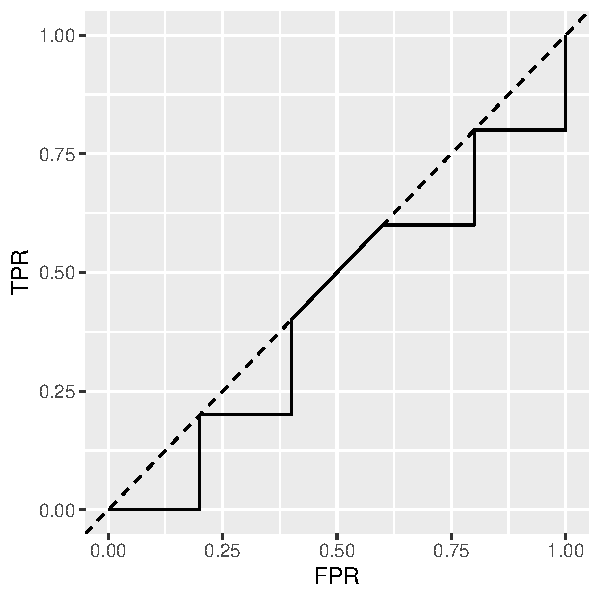
\includegraphics[width=\maxwidth]{figure/unnamed-chunk-11-1} 

}


\end{knitrout}

We see that the resulting ROC lies below the line from the origin with a slope of 1, which represents
a random classifier, i.e., the scoring algorithm performs worse than a random classifier.
If this happens while evaluating the training data, the labels of the scoring algorithm should be inverted.

  \item[d)] 
  We can compute the AUC (\textit{area under the curve}) by looking at the ROC, s.t.
  $$
  AUC = 0.5 - 4 \cdot (0.2 \cdot 0.2 \cdot 0.5) = 0.42.
  $$

\end{enumerate}
}
\end{document}
